\chapter{Event Reconstruction}
\label{sec:event:reco}

The particles produced in the \gls{pp} collisions in the center of the \gls{atlas} detector, interact with the detector material as discussed in Chapter \ref{chap:cern}. As a result of these interactions, electrical currents are recorded. \textit{Event reconstruction} is the process of recombining these digital signals and interpreting them as tracks and energy deposits in the calorimeters. A further step consists in analyzing the characteristics of the candidate tracks and calorimeter clusters and identify them as signs of the passage of specific particles.
This chapter describes the reconstruction and identification of the objects used in the analyses discussed in this thesis: tracks and vertices, electrons, muons, hadronic jets and missing transverse momentum. 


\section{Tracks and Primary Vertices}
\label{sec:reco:tracks}

In \gls{atlas} the identification of tracks from charged particles relies on the information collected by the \gls{id}. The tracking information is crucial to the reconstruction and identification of many types of particles, including electrons, muons, and the jest originating from the hadronization of a b-quark. The precision on the position measurement of the track depends on the granularity of the different subsystems of the \gls{id} and, since the \gls{id} is surrounded by a solenoidal magnetic field, the charged particles follow an helical trajectory. After the point of closest approach (perigee) to a given reference is defined, the trajectory of the track can be described by five parameters: 
\begin{equation}
\theta, \; \phi, \; q/p \; d_0, \; z_0 \;,
\end{equation}
\noindent where $\theta$ and $\phi$ are the azimuthal and polar angle, $q/p$ is the ratio of the charge of the track to the track momentum, and $d_0$ and $z_0$ are the distance to the point of closest approach in the transverse plane and along the $z$-axis. 

Primary tracks, originating from charged particles with a life time longer that $3 \times 10^{-11}$ s produced directly in the hard-scatttering vertex, are reconstructed with an inside-out approach \cite{Cornelissen:1020106}: the seed of the reconstruction are three hits in the silicon detector, and then compatible hits in the outer layers of the \gls{id} are added with a Kalman Filter \cite{citeulike:347166,Fruhwirth:1987fm}. The \gls{trt} segments that are not associated with primary tracks are used as starting point to reconstruct tracks from long-lived particles or from material interaction, with a back-tracking that extrapolates the \gls{trt} information to the pixel hits. 

Random groups of hits can be wrongly reconstructed as belonging to the helical trajectory of a track (\textit{fake tracks}). The amount of fake tracks increases with the increase of pile-up, and can be reduced by tightening the selection criteria of the track, at the expense of reconstruction efficiency. Three different selection criteria are used for the data collected in 2015 and 2016 (Loose, Loose-Primary and Tight-Primary), that differ in the requirements on the hits and holes (elements where a hit was expected but was not registered) in the different \gls{id} layers. The \textit{track reconstruction efficiency} is measured in \gls{mc} simulations as the ratio of the reconstructed tracks matched to a generated charged particle over the total number of generated charged particles. The reconstruction efficiency as a function of the track $\eta$ and \pt is shown in Fig. \ref{fig:obj:tracks} for Loose and Tight-Primary tracks.
 
\begin{figure}[ht]
\centering
\subfigure[]{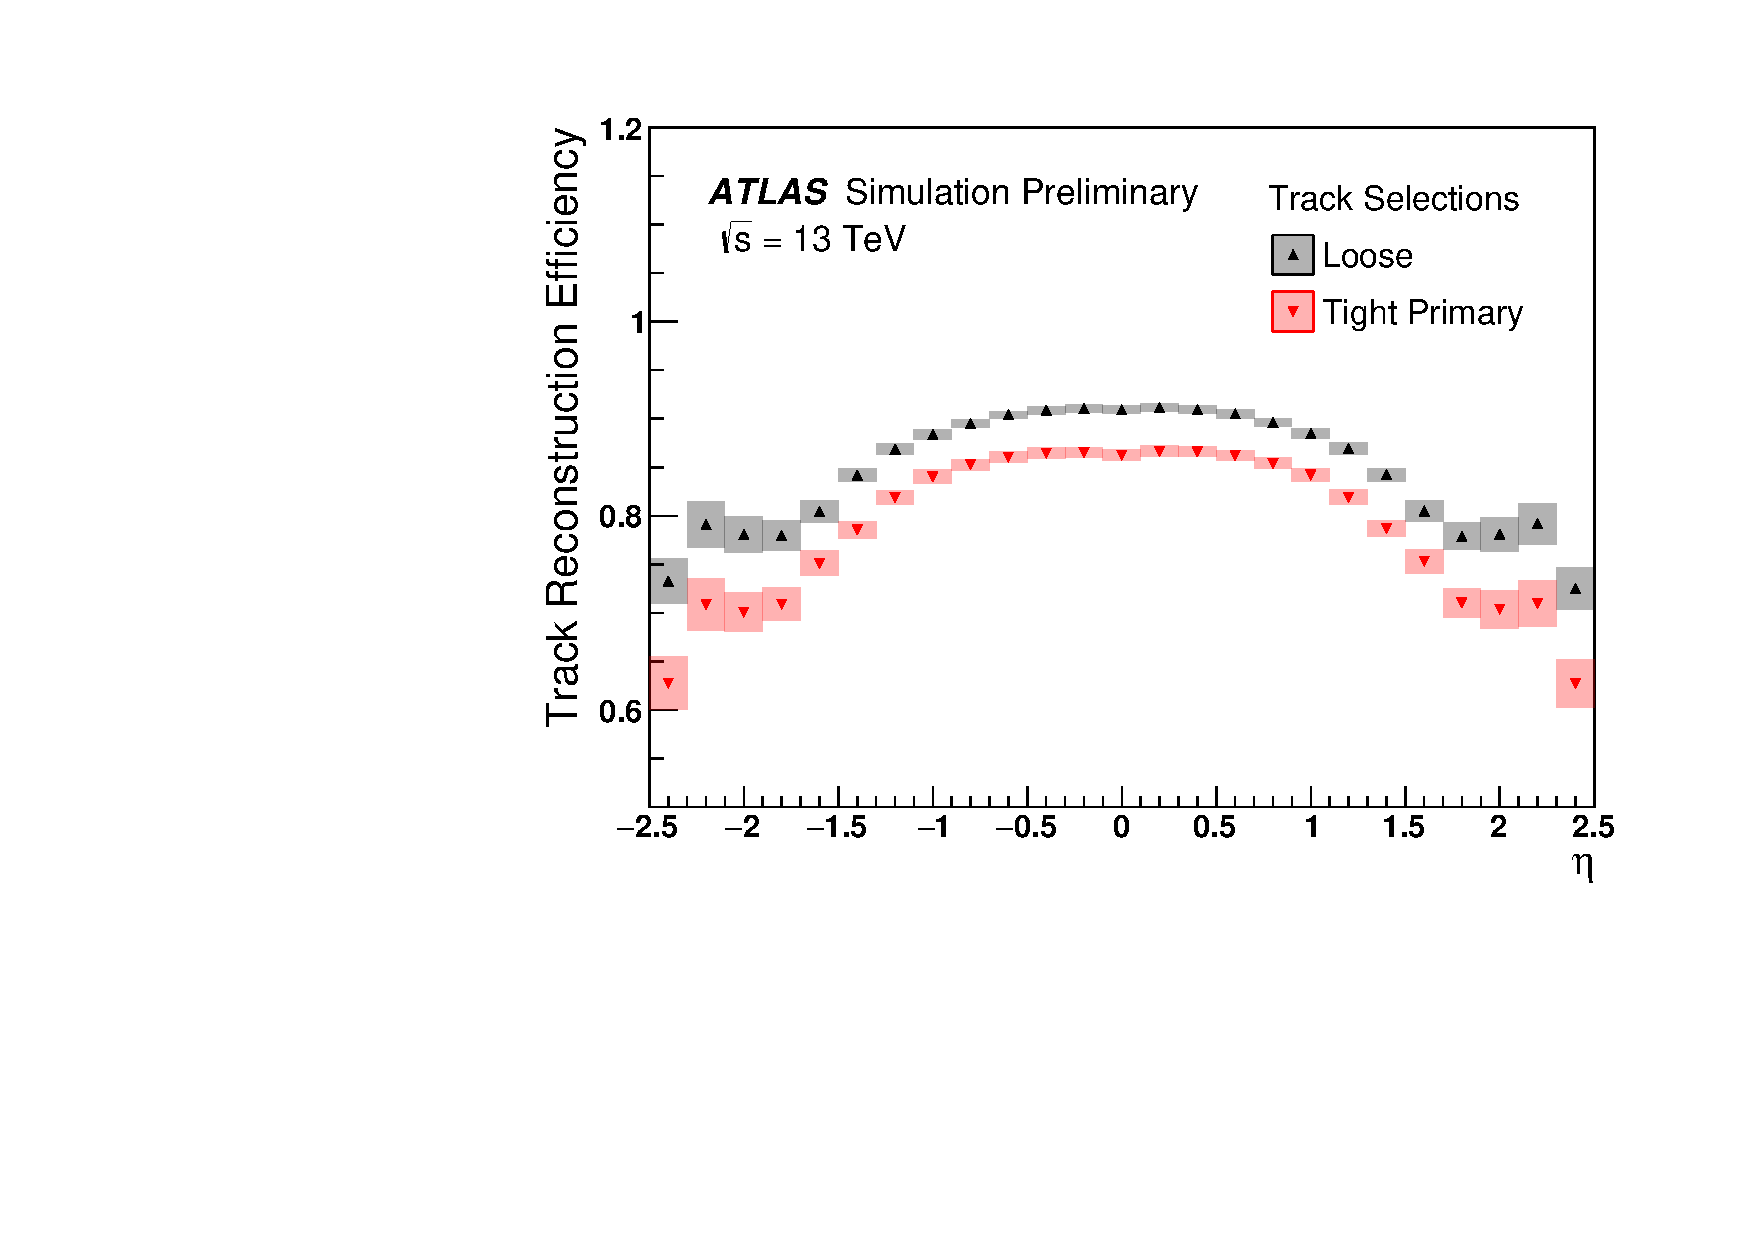
\includegraphics[width=0.48\textwidth]{figures/objects/track1}}
\subfigure[]{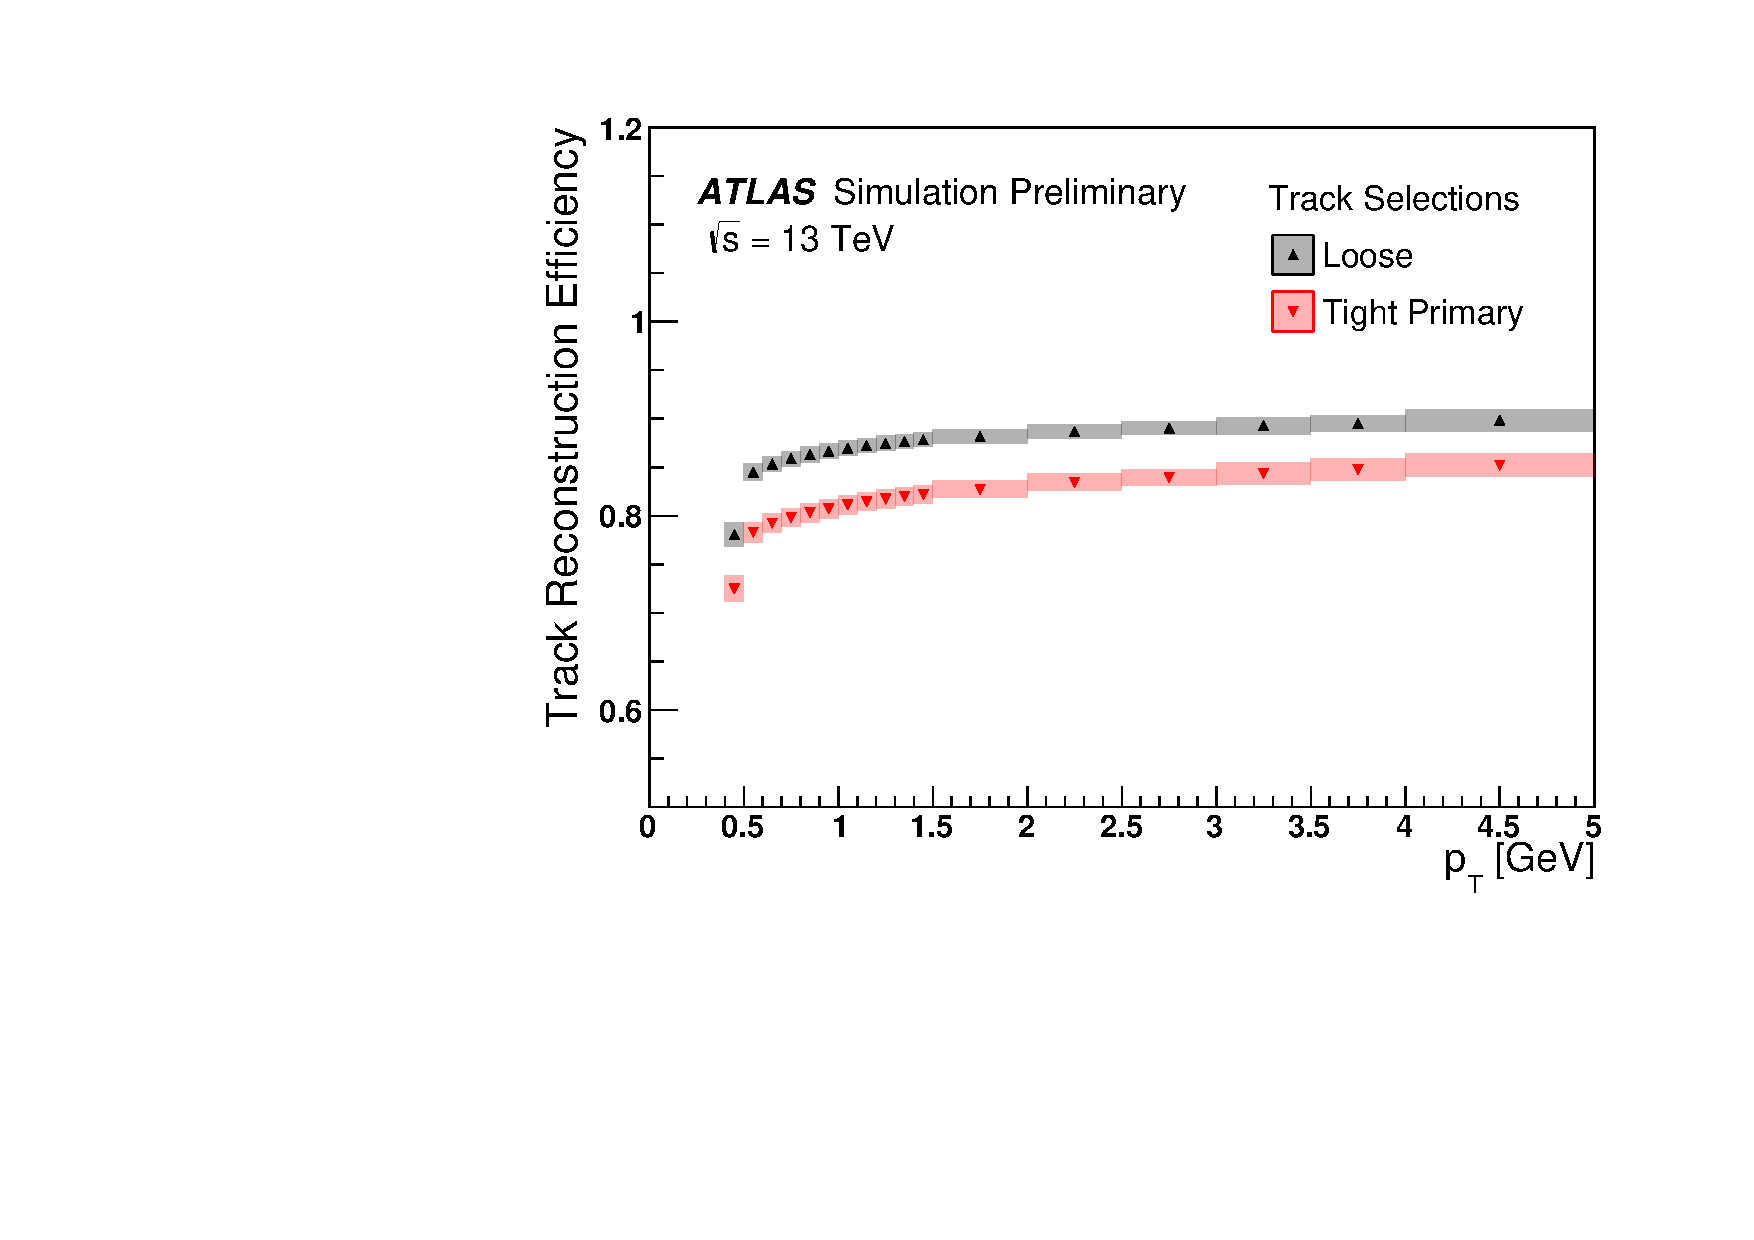
\includegraphics[width=0.48\textwidth]{figures/objects/track2}}
\caption{Track reconstruction efficiency, evaluated by using minimum bias simulated events, as a function of truth $\eta$ (a) and \pt (b) for Loose and Tight Primary track selections.The bands indicate the total sstematic uncertainty. Figure from Ref. \cite{ATL-PHYS-PUB-2015-051}.}
\label{fig:obj:tracks}
\end{figure}

Tracks are the starting point for the identification of vertices. \glspl{pv} are reconstructed through a vertex fitting algorithm \cite{Fruhwirth:2007hz}, and then the vertex fitting algorithm identifies the vertex position and refits the tracks adding the constraint of the reconstructed interaction point. Once all the \glspl{pv} are reconstructed, the one with the highest sum of the squared transverse momenta of its associated tracks ($\sum_i^{N-tracks}p_{T,i}^2$) is identified as the hard scattering vertex, and $d_0$ and $z_0$ are recomputed with respect to its coordinates. The other vertices are named pile-up vertices, and their number is correlated  to the number of interactions per bunch crossing.


\section{Hadronic Jets}

Because of confinement, quarks and gluons produced in the collisions give origin to a collimated spray of hadrons (\textit{jets}) that move in the direction of the original parton. When jets interact with the detector, they loose most of their energy as deposits in the calorimeter systems, which are then grouped together aiming at reconstructing the characteristics of the original parton. 

\subsection{Clusters}
The first step in the jet reconstruction is the procedure that groups the calorimeter cells into topological clusters (\textit{topoclusters}). Topoclusters are built starting from seed cells with a signal-to-noise ratio higher than 4. All the neighboring cells with signal-to-noise ratio higher than two are added with an iterative procedure, and finally a ring of guard cells are added independently of their signal. This procedure is illustrated in Fig. \ref{fig:obj:topocluster}. Topoclusters are calibrated at the \gls{em} scale, which means that the proportionality constant between the readout current and the particle energy is correct only for particles of an \gls{em} shower.

\begin{figure}[h]
\begin{center}
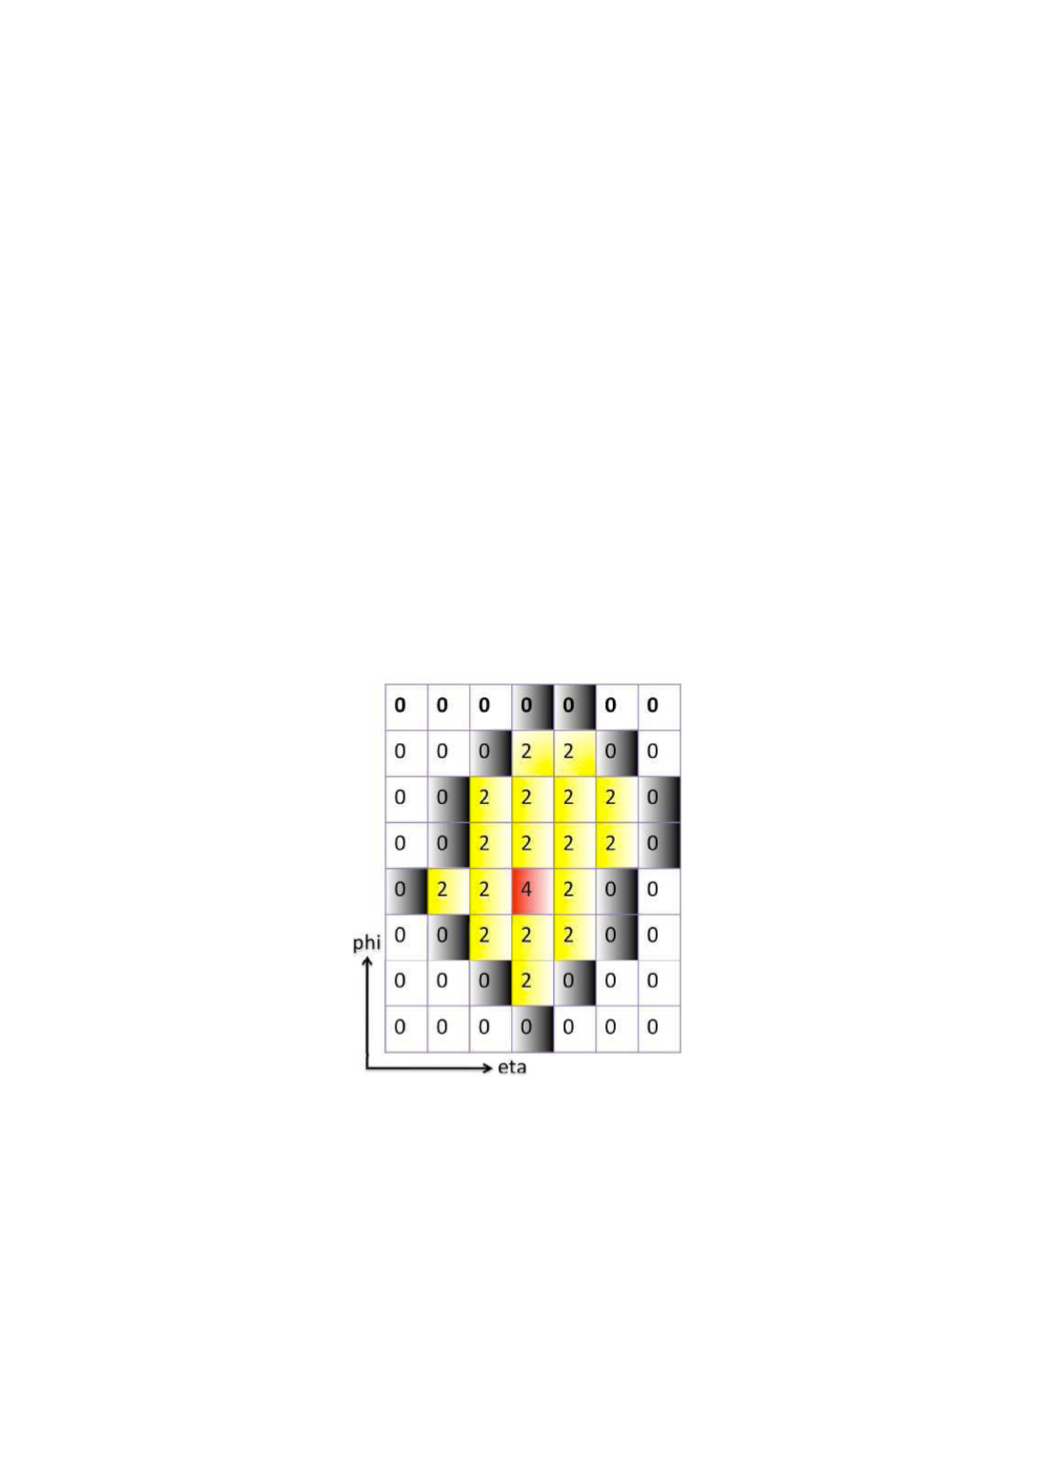
\includegraphics[width=0.3\textwidth]{./figures/objects/topocluster.pdf}
\end{center}
\caption[Topocluster schematic representation]{Topocluster schematic representation. The seed of the cluster is shown in red, the neighbouring cells are in yellow and the ring of guard cells is in grey.}
\label{fig:obj:topocluster}
\end{figure}
 
\subsection{Jet-finding Algorithms}
\label{sec:obj:jetfinding}

The topoclusters are then grouped together by a jet-finding algorithm. Different algorithm are available, and in particular the algorithms of the $k_T$-family merge clusters according to the metric $d_{i,j}$, defined as:

\begin{equation}
d_{i,j} = min\left( k_{T,i}^{2n}, k_{T,i}^{2n}  \right) \frac{\Delta R_{i,j}^2}{R^2},
\label{eq:obj:dij}
\end{equation}

where $k_{T,i}$ is the transverse momentum of the cluster, $\Delta R_{i,j}$ is the angular distance defined as in \ref{eq:deltaR}, $R$ is a fixed parameter, whose values sets the size of the jet, and $n$ is the parameters that defines the kind of algorithm we are using and therefore the shape of the resulting jets. Eq. \ref{eq:obj:dij} defined the distance between two clusters, while the cluster-beam distance is defined as:

\begin{equation}
d_{i,B} =  k_{T,i}^{2n} \; .
\end{equation}

The grouping of the clusters follows an iterative approach:
\begin{enumerate}
\item For each topocluster, the distances $d_{i,j}$ and $d_{i,B}$ are calculated.
\item If, for some $i$ and $j$, $d_{i,j} < d_{i,B}$, group together the two clusters with the smallest $d_{i,j}$
\item Otherwise, if $d_{i,B} < d_{i,j} \, \forall i \neq j $ the $i$-th cluster is defined as a jet.
\item This procedure is iterated until the jet is defined
\end{enumerate}

Depending on the value of the parameter n, we can distinguish different algorithms:
\begin{itemize}
\item $n=0$: Cambridge-Aachen. The grouping of the clusters depends only on geometrical considerations and not on their momentum. 
\item $n=1$: $k_T$ algorithm. Soft clusters are grouped first.
\item $n=-1$: anti-$k_T$ algorithm. Groups hard objects first; the shape of the jets is more regular than in the two previous cases and is a cone of radius R.
\end{itemize}

The choice of a particular algorithm results in different shapes of the jets, represented in fig. \ref{fig:jetsalg}. The standard algorithm used by \gls{atlas} is the anti-$k_T$ algorithm \cite{cacciari:antikt}.

\begin{figure}[h]
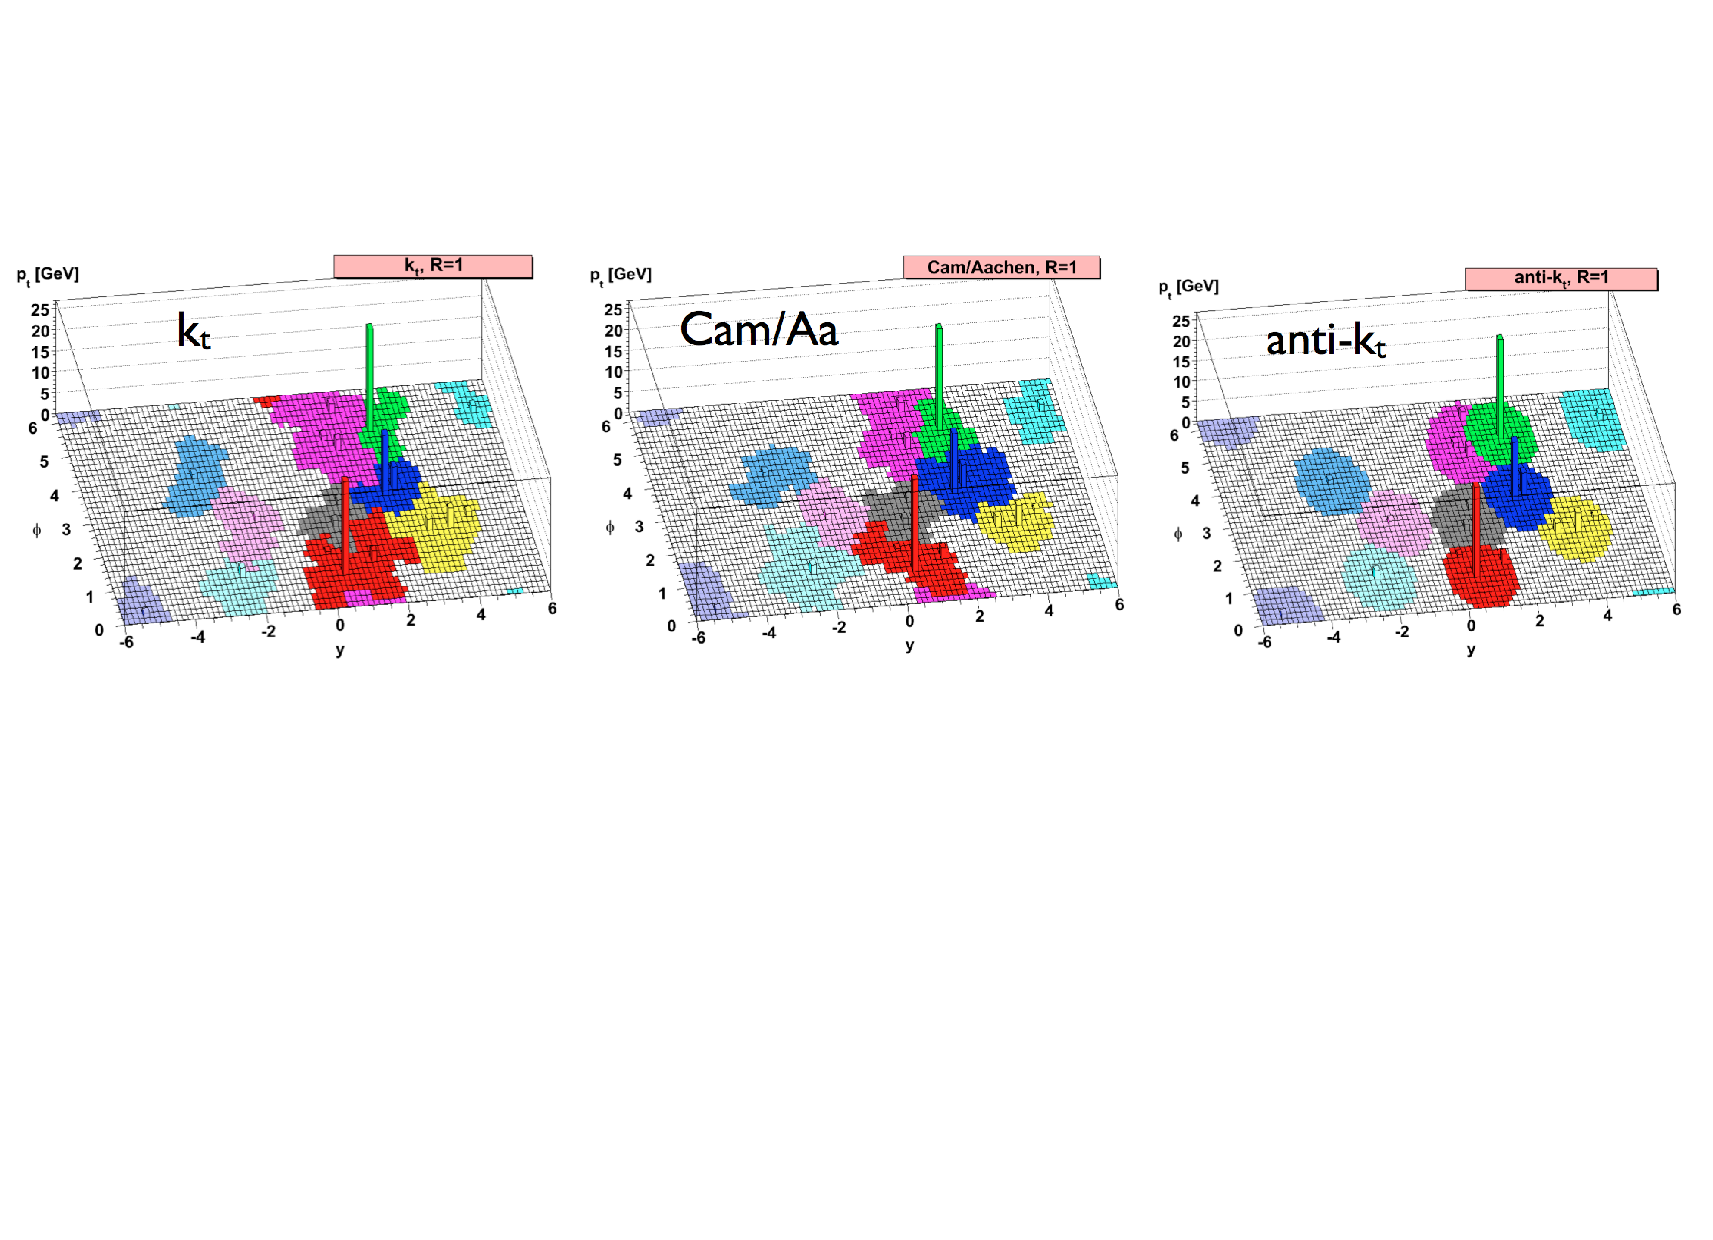
\includegraphics[width=\textwidth]{./figures/objects/jetsalg.pdf}
\caption[Shape of jets reconstructed with different algorithms]{Shape of jets reconstructed with different algorithms \cite{cacciari:antikt}.}
\label{fig:jetsalg}
\end{figure}

\subsection{Jet Calibration}
\label{sec:obj:jetcalib}

As mentioned above, the inputs to the jet-finding algorithms are calibrated at \gls{em} scale, and its coordinate refer to the center of the detector. To access a more precise measurement of the jet energy and kinematics, a sequence of calibration stages are applied; for the 2015-2016 dataset, the standard \gls{atlas} corrections are \cite{PhysRevD.96.072002}:

\begin{description}
\item[Origin correction] The direction of the jet is changed to point at the reconstructed hard-scattering \gls{pv} rather than at the cented of the detector. This correction improves the $\eta$ resolution of the jets.

\item[Pileup correction] Multiple collisions in the same bunch crossing (\textit{in-time pile-up}), as well as residual energy from previous collisions (\textit{out-of-time pile-up}), affect the e jet energy reconstruction. The effect of pile-up is corrected in two steps: a first correction \cite{Cacciari:2007fd,TheATLAScollaboration:2013pia}, dependent on the number of \glspl{pv}, uses the jet area to subtract form the jet energy the average energy form pile-up events. A second correction based on the number of \glspl{pv} and on the number of interactions per bunch crossing, is then applied to disentangle the the effect of in-time pile-uo and out-of-time pile-up.

\item[Absolute calibration] The absolute \gls{jes} and $\eta$ correction is derived comparing in \gls{mc} the truth energy of a jet with the reconstructed energy, and also correct for biases in the $\eta$ reconstruction \cite{Aad2015jets}.

\item[Global sequential calibration] The \gls{gsc} \cite{ATLAS:2015oia} improves the \gls{jes} resolution by deriving additional corrections based on individual jet properties, for example the number of associated tracks and the fraction of energy deposited in the various layers of the calorimeter.

\item[In-situ calibration] As a last stage, the data-driven calibration (\textit{in-situ}) \cite{ATLAS:2015uwa} corrects for the differences between \gls{mc} simulation and data (arising for example from imperfect simulation of the detector response and material interaction). These corrections are derived from events where the jet \pt is balanced against other well measured objects. In the $\eta$-intercalibration, dijet events are used to correct the response of forward jets using well-measured central jets. The response of central jets is instead measured in $Z$+jets, $\gamma$+jets and multijet events. 
 
\end{description}

\subsubsection{Jet Calibration Uncertainties}

The calibration procedure described above implies a set of uncertainties. In particular, 
the \gls{atlas} \gls{jes} Run-2 calibration includes a set of 80 systematic uncertainties; 
67 of those derive from the in-situ calibration \cite{PhysRevD.96.072002}, accounting for modelling uncertainties, 
sample statistics and uncertainties on the calibration of other physics objects used in deriving the calibration. 
The other 13 systematic uncertainties derive from the pileup correction, the $\eta$-intercalibration 
and differences in the jet response and composition for jets of different flavors. 
The full combination of the uncertainties derived from the first 3.2 \ifb of the Run 2 data 
is shown in Fig. \ref{fig:obj:jessyst} as a function of \pt at $\eta = 0$ and as a function of $\eta$ at \pt$ = 80$ GeV.

\begin{figure}[h]
\begin{center}
  \subfigure[]{
    \label{fig:Comb_syst:pt}
    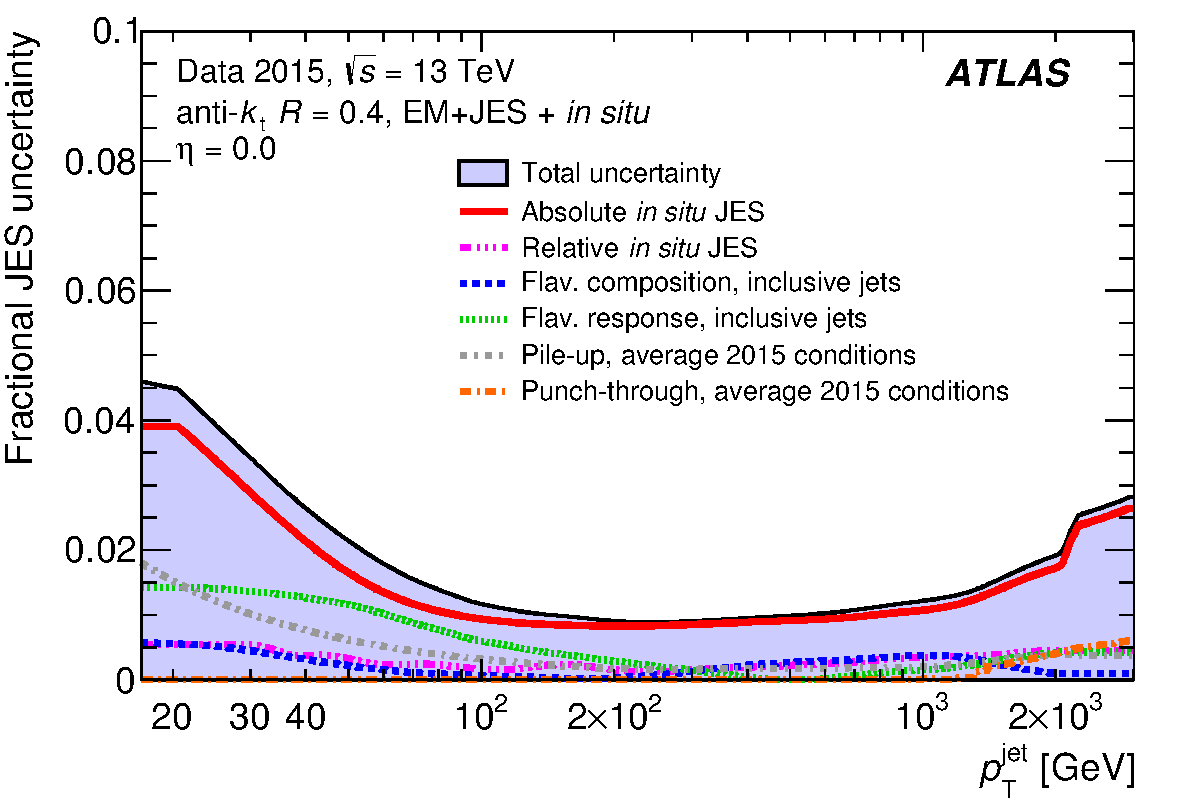
\includegraphics[width=0.48\textwidth]{figures/objects/fig12a.pdf}
  }
  \subfigure[]{
    \label{fig:Comb_syst:eta}
    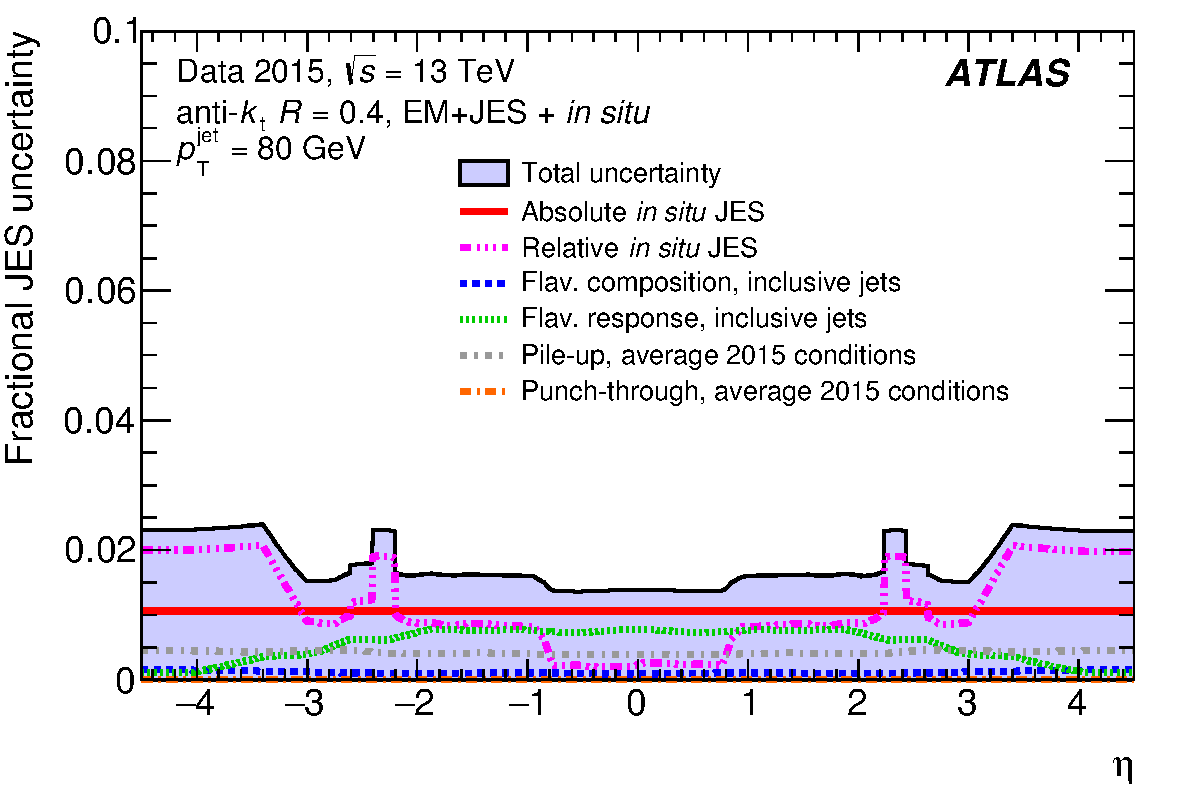
\includegraphics[width=0.48\textwidth]{figures/objects/fig12b.pdf}
  }
\end{center}
 \caption{Combined uncertainty in the \gls{jes} of fully calibrated jets as a function of \subref{fig:Comb_syst:pt}  
 jet \pt at $\eta = 0$ and \subref{fig:Comb_syst:eta} $\eta$ at \pt$ = 80$ GeV. Figure from Ref. \cite{PhysRevD.96.072002}.}
  \label{fig:obj:jessyst}
\end{figure}

To allow an easier usage of the uncertainties in physics analyses, a reduced set of 19 \gls{np} is provided: 
the 67 \glspl{np} from the in-situ calibration are reduced to six by keeping the five uncertainties of largest magnitude, 
plus a sixth one which is the sum in quadrature of the remaining ones. 
A further reduction is in place to group the remaining \glspl{np} into three components, 
and the \glspl{np} within a single component are added in quadrature; this leads to a correlation loss, whose effect is analysis dependent. 

Jets with the same true energy can have different reconstructed energies; the distribution of the difference between true and reconstructed energy of a jet is modeled with a Gaussian, whose width is defined as \gls{jer}. The measurements for the in-situ calibrations can be used also to access the differences in \gls{jer} between data and \gls{mc} \cite{TheATLAScollaboration:2015ofv,ATLAS:2015uwa}, and result into an additional \gls{np}.

\subsection{Jet Vertex Tagger}

It has already been discussed in Sec. \ref{sec:obj:jetcalib} how pileup is taken into account in the calibration of the \gls{jes}. Beside affecting the jet energy, high levels of pileup can also lead to the reconstruction of spurious jets not originating from the hard-scattering interaction. In \gls{atlas} track-based algorithms are used for the identification of pileup jets \cite{Aad:2015ina,ATLAS:2014cva}. 
Tracks are matched to calorimeter jets by ghost-association \cite{Soyez:2012hv}. Once the \gls{pv} is identified, 
for each jet it is possible to compute the \gls{jvf}, the ratio of the scalar sum of the \pt of the tracks associated to the jet and originating from the hard scattering vertex \gls{pv}$_0$ to that of all the associated tracks:

\begin{equation}
 \JVF = \frac{\sum_m{p_{{\rm T}, m}^{{\rm track}}({\rm PV}_0)}}{\sum_n\sum_l  p_{{\rm T}, l}^{{\rm track}}({\rm PV}_n)} \; .
 \label{eq:jvf}
\end{equation} 

\noindent where the index $n$ runs over all the vertices of the event. In high-pileup conditions the denominator in 
Eq. \ref{eq:jvf} increases; to correct for this dependence, the \gls{cjvf} is introduced. 
This is a modified version of \gls{jvf}, that takes into account the dependence on the number of pileup tracks (\nPUtrk):

\begin{equation}
\cJVF = \frac{\sum_m{p_{{\rm T}, m}^{{\rm track}}({\rm PV}_0)}}{\sum_l p_{{\rm T}, l}^{{\rm track}}({\rm PV}_0) + \frac{\sum_{n\geq1}\sum_l p_{{\rm T}, l}^{{\rm track}}({\rm PV}_n)}{ (k \cdot \nPUtrk)}} \; ,
\label{eq:corrJVF}
\end{equation}

\noindent with $k=0.001$. Another variable used to discriminate hard-scattering jets against pileup jets is the ratio of the scalar
sum of the \pt of the tracks originating from \gls{pv}$_0$ to the jet transverse momentum:


\begin{equation}
\RpT = \frac{\sum_k{p_{\rm{T}, k}^{{\rm track}}({\rm PV}_0)}}{\ptjet}
\end{equation}

The \cJVF and \RpT are combined in a two-dimensional likelihood that constitutes a single tagger, the \gls{jvt}. 

\begin{figure}[h]
\begin{center}
  \subfigure[]{
    \label{fig:obj:jvt_mc}
    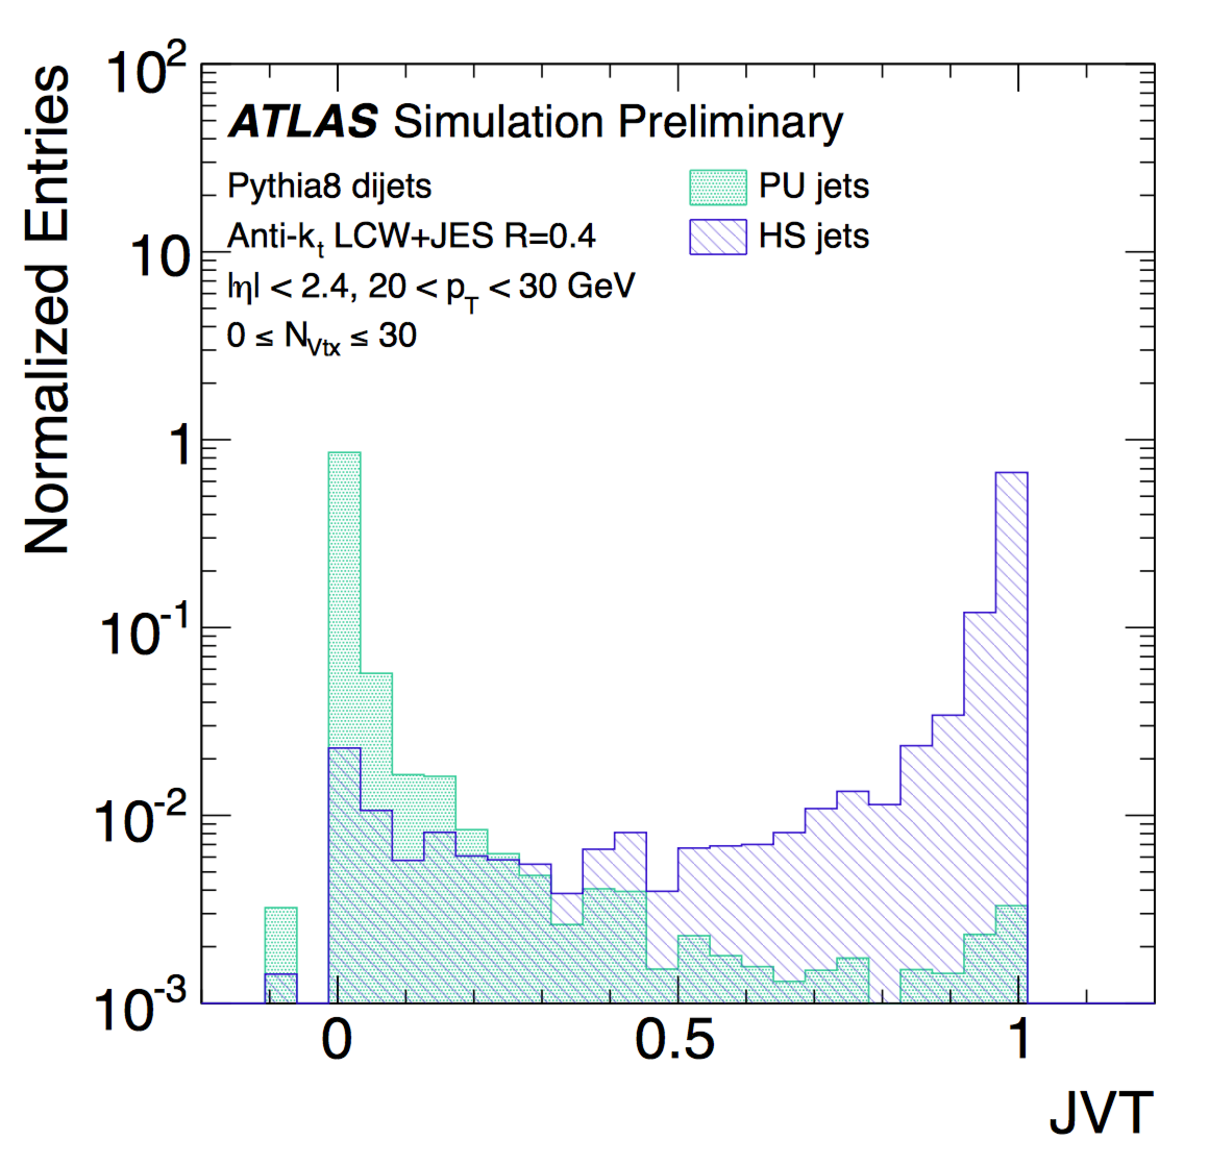
\includegraphics[width=0.48\textwidth]{figures/objects/jvt.pdf}
  }
  \subfigure[]{
    \label{fig:obj:jvt_data}
    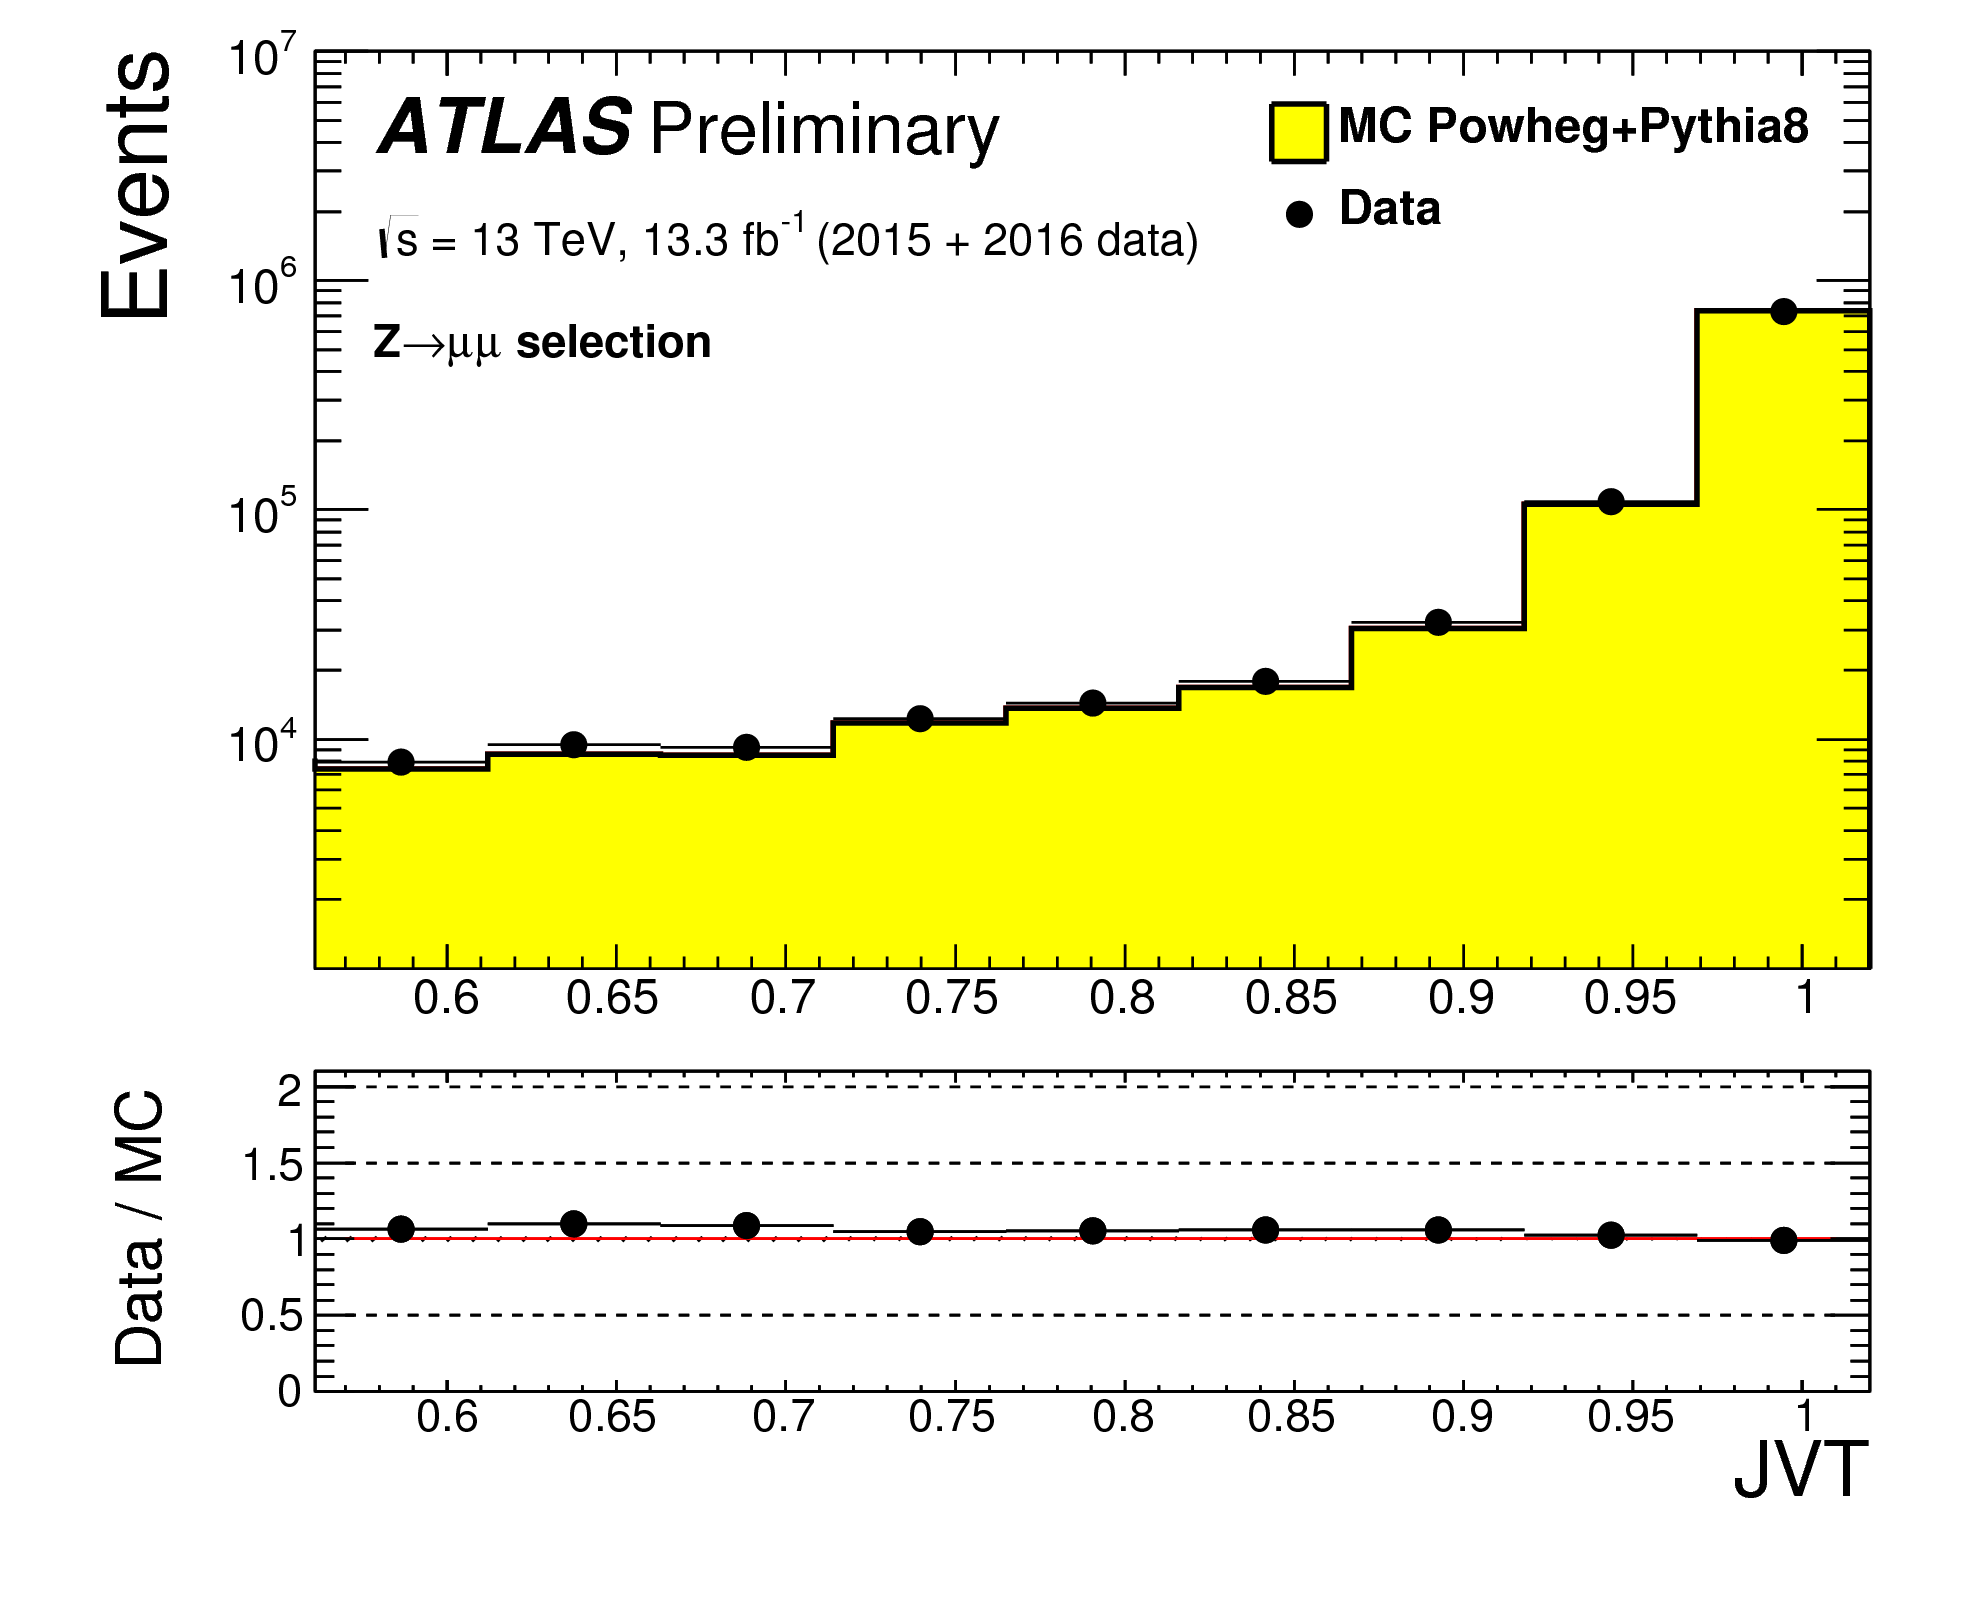
\includegraphics[width=0.48\textwidth]{figures/objects/jvt_data.png}
  }
\end{center}
 \caption{\subref{fig:obj:jvt_mc} Distribution of JVT for pileup and hard-scatter jets with 20 < \pt < 30 GeV. Figure from Ref. \cite{ATLAS:2014cva}. \subref{fig:obj:jvt_data} The JVT distribution, in Powheg+Pythia8 MC and in 2015+2016 data, of jets balanced against Z bosons decaying to muons. Figure from Ref. \cite{jvtpublicplots}.}
  \label{fig:obj:jvt}
\end{figure}

\subsection{Jet Cleaning}

\subsection{Re-clustered Jets}

The angular separation between the decay products of a particle with mass $m^P$ and transverse momentum 
$p_T^P$ scales as:
\begin{equation}
\Delta R \approx \frac{2 m^P}{p_T^P} \; .
\end{equation}

This indicates that the ideal value of the $R$ parameter described in Sec. \ref{sec:obj:jetfinding} can vary depending on the event topology that we want to capture;
for example, the decay products of an heavy particle with a transverse momentum much larger than its rest mass (\textit{boosted object}) could be better described by a 
single jet with a larger $R$ than with multiple jets with the "standard" 0.4 radius, 
as it happens for example in the decay of very energetic top quarks, W, Z or Higgs bosons produced at the LHC.
Each different value of the $R$ parameter requires a dedicated calibration following the steps described in Sec. \ref{sec:obj:jetcalib}. 
Therefore, it is not always possible to choose the optimal value of the jet radius. 
A possible solution to this problem comes from noticing that the same jet-finding algorithms used to group topoclusters can have different types of inputs. 
In particular, jets themselves can be be used as input and grouped together, and in this case we speak of \textit{re-clustered jets} \cite{Nachman:2014kla}. 
The re-clustered jest are automatically calibrated as long as the input jets are, and also the jet uncertainties can be propagated directly. 
A comparison of the jet clustering obtained with $R$=1.0 anti-$k_T$ and by re-clustering anti-$k_T$ $R$=0.3 jets into anti-$k_T$ $R$=1.0
is shown in Fig. \ref{fig:recluster}. It is possible to see how the jet axis is similar between the two cases, and how the $R$=1.0 anti-$k_T$ have more inputs away from the jet axis.
Re-clustered jets can be \textit{trimmed} by removing the constituent small-R jets that have a \pt smaller than a defined fraction of the \pt of the original reclustered jet. 


\begin{figure}[h]
\begin{center}
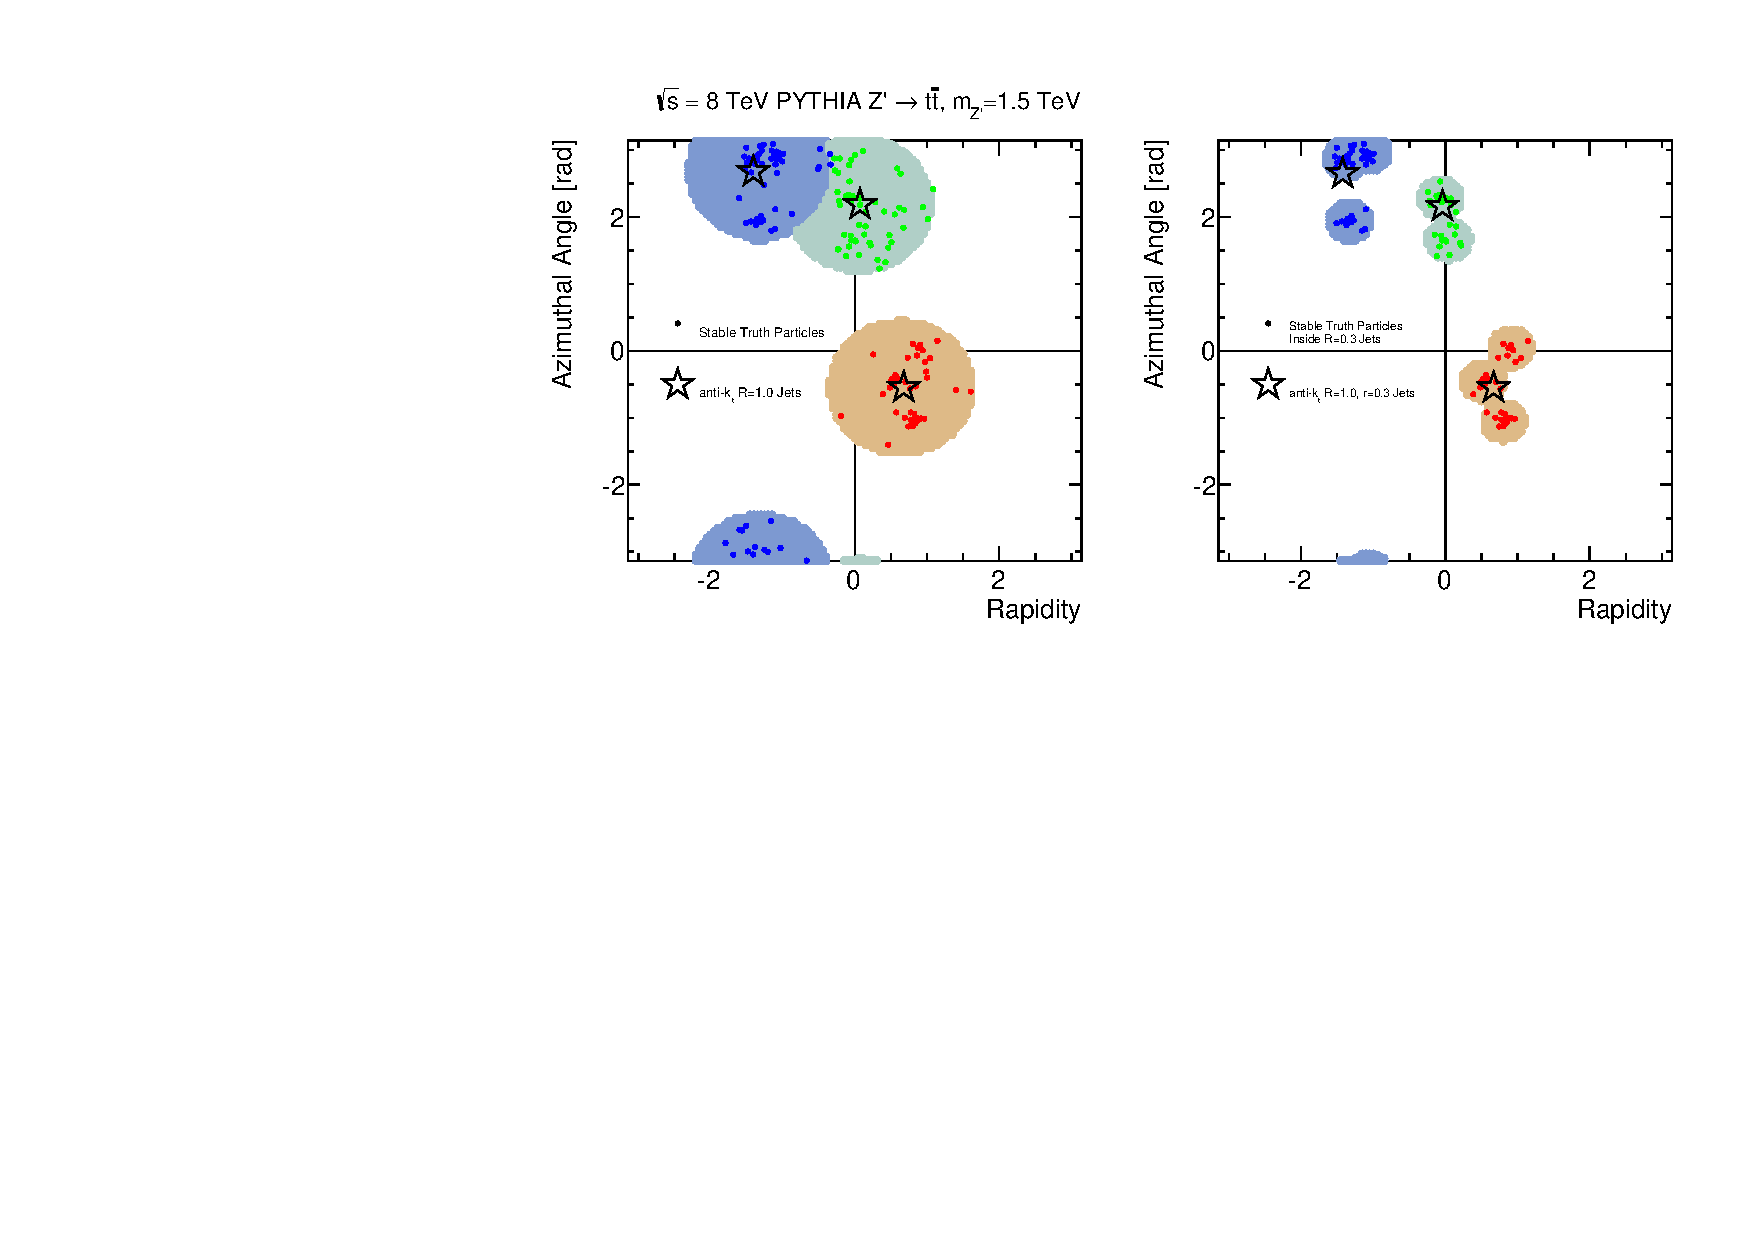
\includegraphics[width=1.0\textwidth]{./figures/objects/reclustered.pdf}
\end{center}
\caption{Example event where jets have been clustered with (a) anti-$k_T$ with $R$=1.0 and (b) anti-$k_T$ $R$=1.0 re-clustered jets (starting from anti-$k_T$ $R$=0.3 jets); the shaded region shows the jet area. Figure from Ref. \cite{Nachman:2014kla}.}
\label{fig:recluster}
\end{figure}

\section{Jets from B-hadrons}

Jets originating from the hadronization of a b-quark (b-jets) can be identified thanks to the lifetime of B-hadrons (about $10^{-12}$ s), which is shorter than the typical lifetime of hadrons containing only light quarks, but still long enough to allow the B-hadrons to travel distances of the order of the mm before decaying. A schematic view of the topology originating from a jet containing a B-hadron is shown in Fig. \ref{fig:btag}.


\begin{figure}[h]
\begin{center}
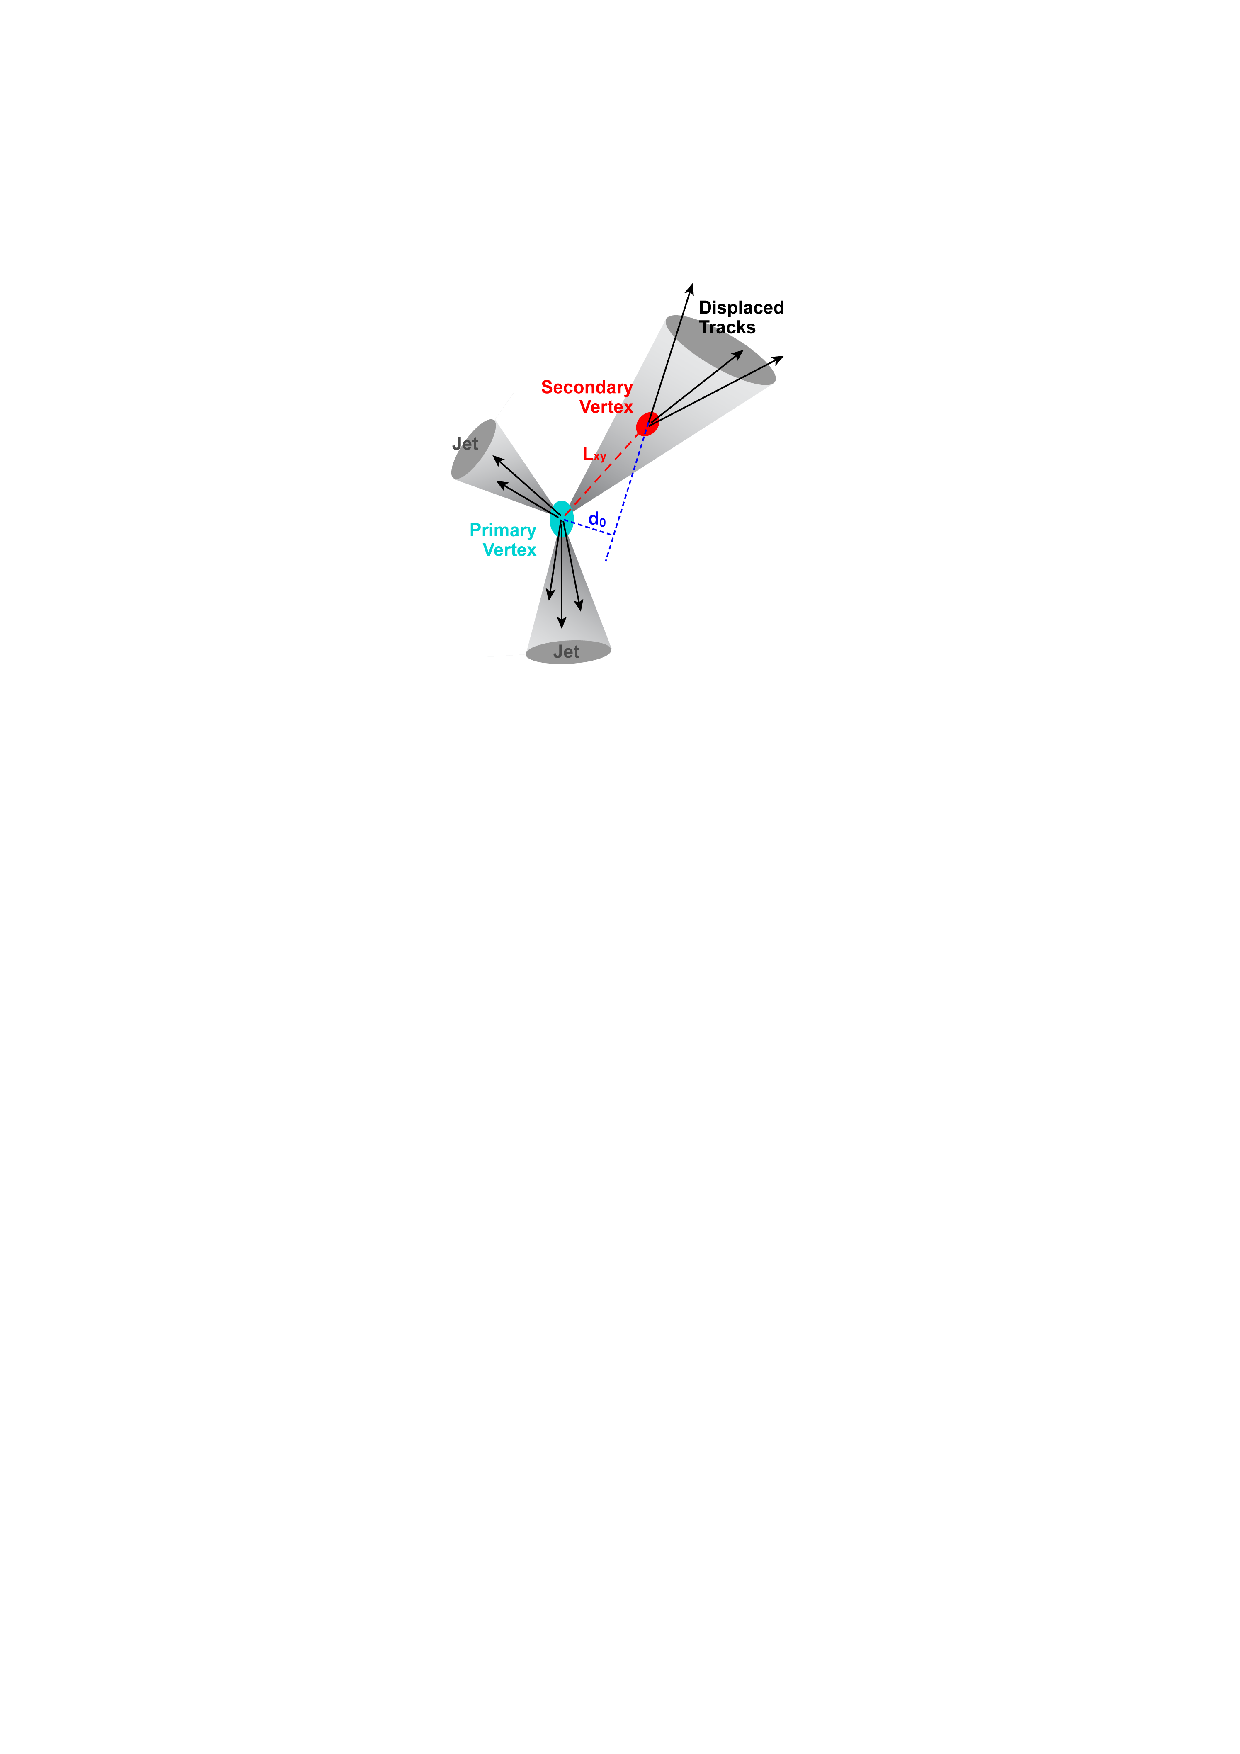
\includegraphics[width=0.45\textwidth]{./figures/objects/secvtx.pdf}
\end{center}
\caption[Schematic view of the topology of a b-jet.]{Schematic view of the topology of a b-jet. Figure from Ref. \cite{d0btagging}.}
\label{fig:btag}
\end{figure}

\subsection{B-tagging Calibration and Uncertainties}


\section{Electrons}

\section{Muons}

\section{Missing Transverse Momentum}

Particles that interact only weakly with the detector, such as neutrinos or BSM particles like neutralinos, are not reconstructed directly. 
Their presence is instead inferred by measuring the total momentum imbalance in the event. 

\begin{equation}
\met = \sqrt{(E_{X}^{miss})^{2}  +  (E_{Y}^{miss})^{2}},
\end{equation}

\begin{equation}
E_{X(Y)}^{miss} = E_{X(Y)}^{miss,e} +    E_{X(Y)}^{miss,\gamma} + E_{X(Y)}^{miss,\tau}    \nonumber \\
+ E_{X(Y)}^{miss,jets} + E_{X(Y)}^{miss,soft-terms}  +  E_{X(Y)}^{miss,\mu} 
\label{eq:etm} 
\end{equation}


\begin{equation}
\phi^{miss} = \arctan \left( \frac{E_Y^{miss}}{E_X^{miss}} \right)
\end{equation}




